\documentclass{beamer}

\mode<presentation> {
\usetheme{Copenhagen} % Pretty neat, soft color.
\setbeamercovered{transparent}
\setbeamercovered{invisible}
\setbeamertemplate{navigation symbols}{} 
}

\usepackage{graphicx,amssymb}
\usepackage{amsmath}
\usepackage{bm} 
\usepackage{wasysym}

\title[ECML/PKDD 2011 demo session (demo \#10)]{InFeRno - an Intelligent Framework for Recognizing Pornographic Web pages}
\author{\bf{\underline{S. Karavarsamis}, N. Ntarmos and K. Blekas }}

\institute[UoI]
{\large
Department of Computer Science\\
University of Ioannina, Ioannina, Greeece \\
\medskip
{\normalsize E-mail: \{cs061205, ntarmos, kblekas\}@cs.uoi.gr}
}
\date{}

\begin{document}

\begin{frame}
\titlepage
\end{frame}

\begin{frame}
\frametitle{Problem preliminaries and intuition}

\begin{itemize}
	\item Leverage human intervention in content assessment

	\begin{enumerate}
		\item Demanding need for intelligent content assessment
		\item Content too diverse and enormous to pre-classify manually
	\end{enumerate}

	\item Nudity-content indicator cues
	
	\begin{enumerate}
		\item exploit accompanying text (prior knowledge)
		\item visual content (images, video, audio)
	\end{enumerate}
	
	\item Web page assessment based solely on the image content

	\begin{enumerate}
		\item Determine an efficient feature vector space
		\item Introduce an intermediate 'bikini' class
		\item Facilitate identification of 'soft' nudity
		\item Employ multi-class SVM in a one-against-all scheme
		\item Provide full-fledged pornography elimination system implementation (ICAP/HTTP proxy integration)
	\end{enumerate}
\end{itemize}

\end{frame}

\begin{frame}
\frametitle{InFeRno architecture}
\begin{center}
	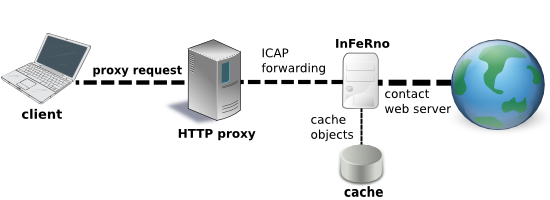
\includegraphics[scale=0.6]{images/network_diagram.png}
	\begin{enumerate}
		\item The administrator can tweak classification / network parameters (flexible configuration)
		\item Standalone implementation of the InFeRno core as an ICAP module (integrates well with most HTTP proxy servers)
		\item Decoupled image classification and web page preprocessing (network I/O, web page fusion)
		\item Using a fast ISAM-based cache for fast  I/O (classification lookups, updates, etc)
	\end{enumerate}
\end{center}
\end{frame}

\begin{frame}
\frametitle{Image classification}
\begin{center}
		\begin{tabular}[c]{ccc}
		\ \ 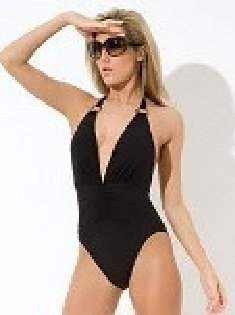
\includegraphics[width=.13\columnwidth]{images/orig.pdf}  \ \ &
		\ \ 
\includegraphics[width=.13\columnwidth]{images/skin.pdf} \ \ &
		\ \ 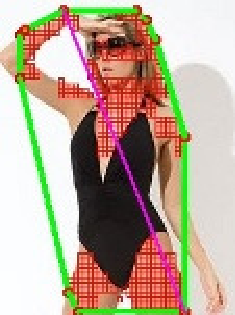
\includegraphics[width=.13\columnwidth]{images/grid.pdf} \ \ \\
			original image & skin detection & contour extraction \\
		\end{tabular}
\end{center}

\begin{itemize}
  \item 3-stage image processing/classification
     \begin{enumerate}
        \item Image preprocessing, and skin detection (pixel-based)
        \item Contour extraction (rough ROI estimation)
		\item Feature extraction and Classification
		  \begin{itemize}
			\item Selected Features (mean RGB intensities/deviations, skin-to-nonskin ratio, contour orienation, Hu moments)
	        \item Classification scheme (multi-class one-against-all SVM scheme employing linear/RBF kernels)
	       \end{itemize}
	\end{enumerate}
   \item Some key-software used in this module
      \begin{enumerate}
		\item OpenCV (mainly image I/O);  libsvm (SVM training); GDK library (GIF support)
	  \end{enumerate}
\end{itemize}
\end{frame}

\begin{frame}
\frametitle{InFeRno vs POESIA}
	\begin{itemize}
		\item Dataset
			\begin{enumerate}
				\item Manually collected a dataset of 680 bikini images, 660 porn images and 4260 benign images from the Web
			\end{enumerate}

		\item Comparison to the POESIA filter (poesia-filter.org)
			\begin{enumerate}
				\item compared InFeRno image filter to that of the POESIA filter in terms of CPU consumption, and generalization ability
			\end{enumerate}
	\end{itemize}
	
	\begin{block}
	{}
	A \textbf{4x speedup} was observed on our dataset (comprising porn, bikini and benign images).
	\end{block}

	\begin{center}
		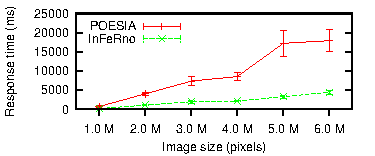
\includegraphics[scale=1.3]{images/scatter-p-t-all-bars.pdf}
	\end{center}

\end{frame}

\begin{frame}
	\centerline{Thank you for your attention! \smiley}
	\centerline{}
	\centerline{\small{visit InFeRno at \bf{github.com/ntarmos/InFeRno}}}
\end{frame}

\end{document} 
